% ===========================================================================
\section{Quantitative results}\label{sec:results}
% ===========================================================================
\subsection{Certified operation versus baselines}
Table~\ref{tab:main} compares all policies at $\alpha=0.05$. Always-aggressive operation on the highest satellite delivers \RAAGood{}\,Mbit per epoch but loses \RAAMiss\% of critical messages, because every misjudged link becomes a deadline miss. Always-robust operation reduces misses to \RARMiss\% but cuts goodput to \RARGood{}\,Mbit and raises energy per delivered megabit to \RAREnergy{}\,J. SeaSel accepts \RSCov\% of epochs with a selective risk of \RSRisk\%, misses \RSMiss\% of critical messages, \RMissRed\% fewer than always-aggressive operation, and delivers \RSGood{}\,Mbit per epoch, \RGoodRatio{} times the goodput of always-robust operation and the same goodput as always-aggressive operation (Fig.~\ref{fig:pareto}). Its selective risk exceeded the target in only \RSViol{} of the 100 calibration/test splits, well within the guaranteed $\delta=0.10$.

\begin{table}[t]\centering\small
\caption{\textbf{Main results on the held-out pool} (target $\alpha=0.05$, $\delta=0.1$; mean $\pm$ s.d. over 100 random calibration/test splits). Viol.: fraction of splits with selective risk above $\alpha$.}
\label{tab:main}
\resizebox{\textwidth}{!}{\begin{tabular}{@{}lccccccc@{}}\toprule
Method & Certified & Coverage & Selective risk & Miss rate & Goodput & Energy & Viol.\\
 & & & & (\%) & (Mbit/epoch) & (J/Mbit) & \\\midrule
Max-elevation (always aggressive) & no & 1.000 $\pm$ 0.000 & 0.133 $\pm$ 0.001 & 13.29 $\pm$ 0.11 & 348.9 $\pm$ 0.4 & 0.57 $\pm$ 0.00 & 1.00\\
Always robust (dual diversity) & no & 0.000 $\pm$ 0.000 & 0.000 $\pm$ 0.000 & 1.19 $\pm$ 0.04 & 19.8 $\pm$ 0.0 & 20.13 $\pm$ 0.01 & 0.00\\
Link-budget margin, tuned & no & 0.343 $\pm$ 0.002 & 0.051 $\pm$ 0.001 & 6.52 $\pm$ 0.09 & 142.4 $\pm$ 0.6 & 2.31 $\pm$ 0.01 & 0.81\\
Logistic regression, tuned & no & 0.919 $\pm$ 0.001 & 0.054 $\pm$ 0.001 & 5.94 $\pm$ 0.07 & 350.8 $\pm$ 0.4 & 0.61 $\pm$ 0.00 & 1.00\\
Gradient boosting, tuned & no & 0.936 $\pm$ 0.001 & 0.062 $\pm$ 0.001 & 6.80 $\pm$ 0.08 & 353.8 $\pm$ 0.4 & 0.60 $\pm$ 0.00 & 1.00\\
Gradient boosting + LTT & yes & 0.898 $\pm$ 0.003 & 0.046 $\pm$ 0.002 & 5.23 $\pm$ 0.15 & 346.0 $\pm$ 0.5 & 0.63 $\pm$ 0.00 & 0.01\\
PBA single model + LTT & yes & 0.900 $\pm$ 0.002 & 0.046 $\pm$ 0.001 & 5.26 $\pm$ 0.13 & 346.5 $\pm$ 0.5 & 0.63 $\pm$ 0.00 & 0.02\\
\textbf{SeaSel (PBA ensemble + LTT)} & yes & 0.906 $\pm$ 0.002 & 0.046 $\pm$ 0.001 & 5.21 $\pm$ 0.14 & 349.0 $\pm$ 0.5 & 0.62 $\pm$ 0.00 & 0.01\\
\bottomrule\end{tabular}}\end{table}

The uncertified baselines show why certification is needed. Thresholds tuned on validation data look adequate during tuning but exceed the target on new data: gradient boosting with a tuned threshold reaches a selective risk of \RGTRisk\% and violates the target in \RGTViol{} of the splits; logistic regression behaves the same way, and the link-budget heuristic violates it in 81\% of splits while accepting only a third of the epochs. Applying the SeaSel certificate to the same gradient-boosting predictor removes the violations (selective risk \RGRisk\%, coverage \RGCov\%). The certificate is therefore model-agnostic, and the guarantee comes from the certification layer rather than from any particular predictor.

\begin{figure}[t]
\centering
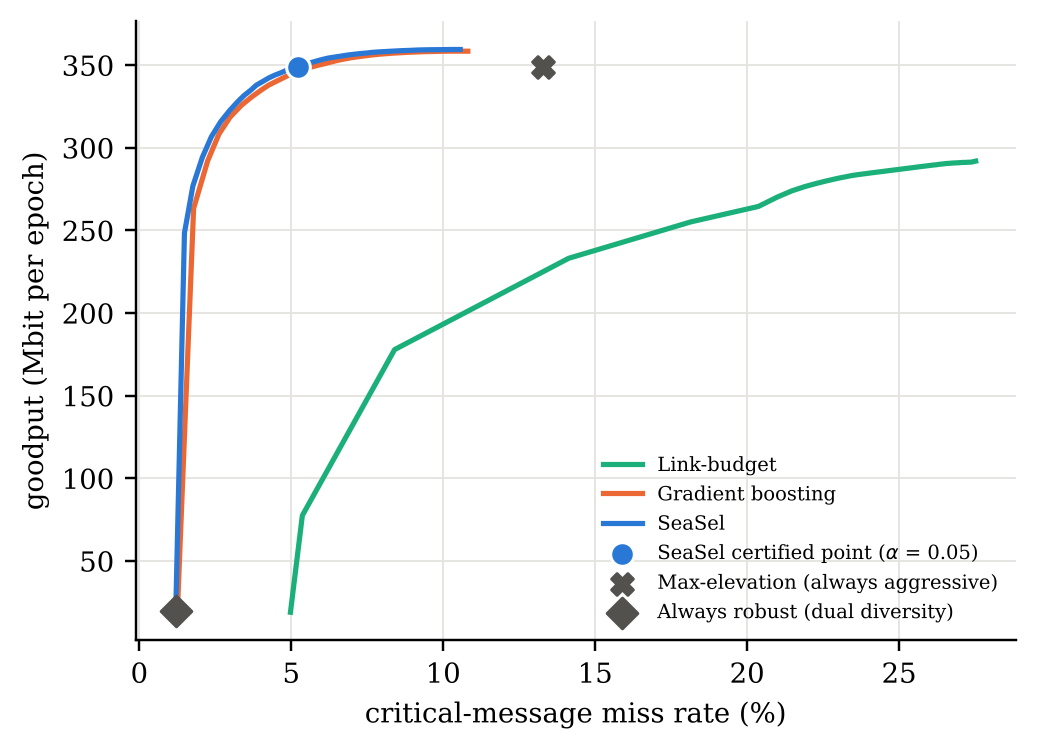
\includegraphics[width=0.62\textwidth]{../figures/fig_pareto.png}
\caption{\textbf{Goodput against critical-message miss rate.} Curves sweep the acceptance threshold; markers show the certified SeaSel operating point and the two fixed policies. SeaSel matches always-aggressive goodput while removing most of its misses.}
\label{fig:pareto}
\end{figure}

\subsection{Prediction quality and calibration}
Table~\ref{tab:disc} and Fig.~\ref{fig:riskcov} report discrimination and calibration. The SeaSel ensemble attains the highest AUROC (\RSAuroc), the lowest calibration error (\RSEce{} against \RGEce{} for gradient boosting) and the lowest area under the risk--coverage curve (\RSAurc). Its margin in AUROC over the strongest tabular baseline is small (\RSAuroc{} against \RGAuroc), so in-distribution gains in coverage are modest: SeaSel certifies \RCovGain{} percentage points more epochs than gradient boosting with the same certificate. The reliability diagram (Fig.~\ref{fig:reliability}) shows that the ensemble probabilities lie close to the diagonal, which matters because the uncertainty-penalised score (\ref{eq:choice}) uses them directly. The physics-free link-budget heuristic reaches an AUROC of only \RLAuroc, which confirms that motion, weather and history must be learned jointly.

\begin{table}[t]\centering\small
\caption{\textbf{Discrimination and calibration of the link-success predictors} on the held-out pool.}
\label{tab:disc}
\begin{tabular}{@{}lccc@{}}\toprule
Predictor & AUROC $\uparrow$ & ECE $\downarrow$ & AURC $\downarrow$\\\midrule
Link-budget margin & 0.684 & 0.209 & 0.1146\\
Logistic regression & 0.903 & 0.009 & 0.0134\\
Gradient boosting & 0.901 & 0.020 & 0.0135\\
PBA single model & 0.901 & 0.010 & 0.0136\\
SeaSel ensemble & 0.907 & 0.005 & 0.0126\\
\bottomrule\end{tabular}\end{table}

\begin{figure}[t]
\centering
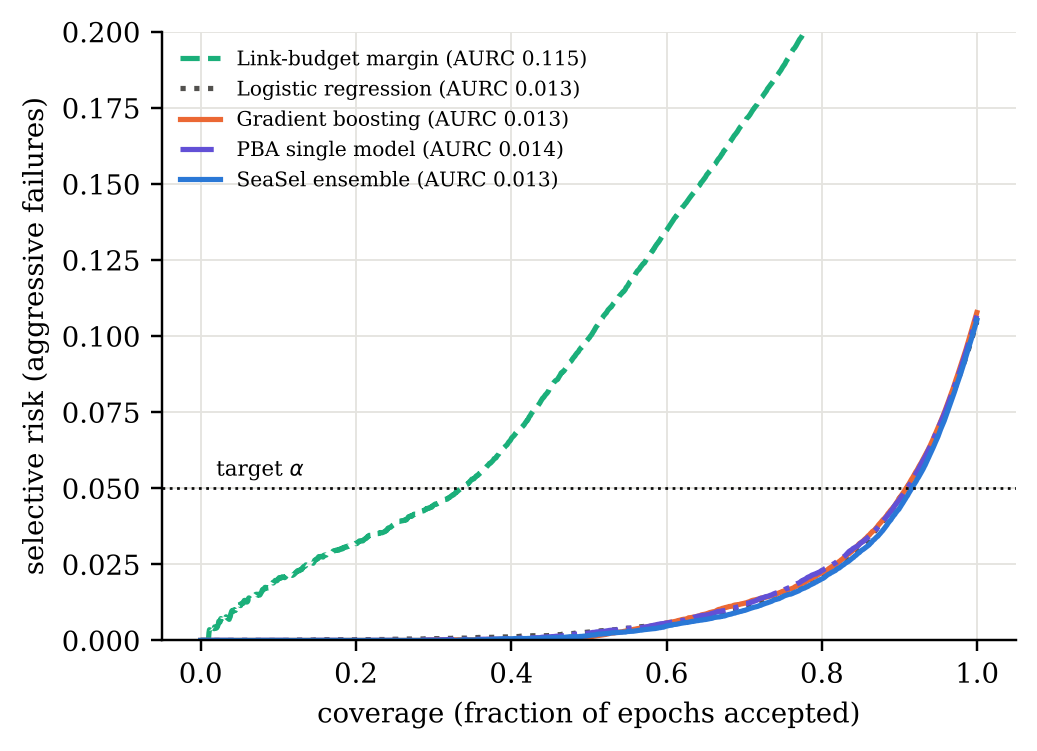
\includegraphics[width=0.6\textwidth]{../figures/fig_risk_coverage.png}
\caption{\textbf{Risk--coverage curves of the link predictors.} Selective risk of aggressive transmissions as a function of the fraction of accepted epochs.}
\label{fig:riskcov}
\end{figure}

\begin{figure}[t]
\centering
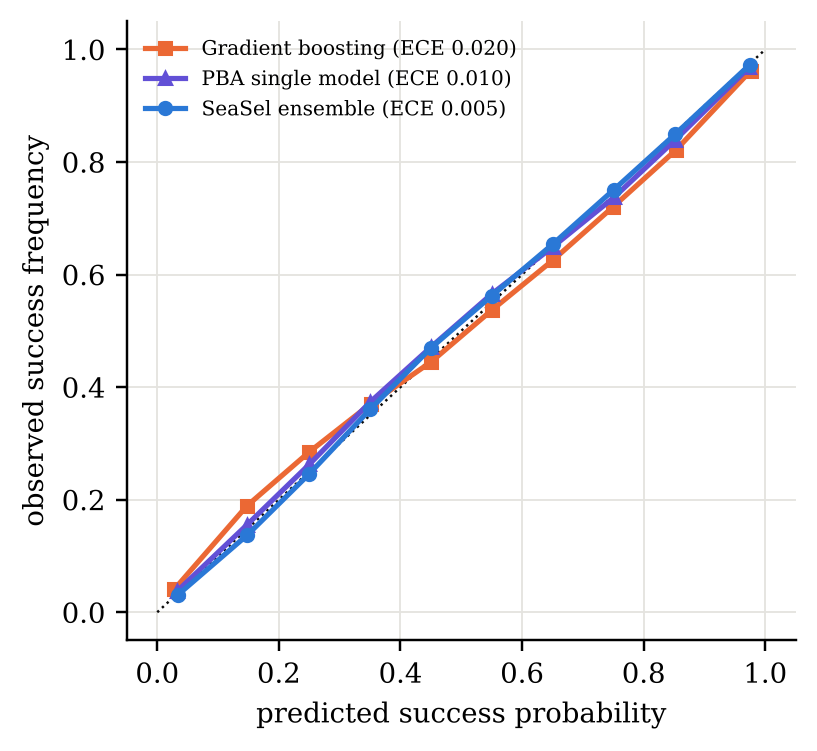
\includegraphics[width=0.5\textwidth]{../figures/fig_reliability.png}
\caption{\textbf{Reliability diagram.} Observed against predicted success probability on the evaluation pool.}
\label{fig:reliability}
\end{figure}

\subsection{Validity of the guarantee across risk targets}
Figure~\ref{fig:alpha} varies the target from $\alpha=0.02$ to $0.15$. With certification, the realised selective risk stays at or below the diagonal for every target, and the violation frequency never exceeds 0.04 for either SeaSel or certified gradient boosting. The tuned threshold lies above the diagonal for all targets up to 0.08 and violates them in every split. Certification costs coverage only where it should: at $\alpha=0.02$ SeaSel accepts 77\% of epochs, and coverage approaches 99\% at $\alpha=0.10$.

\begin{figure}[t]
\centering
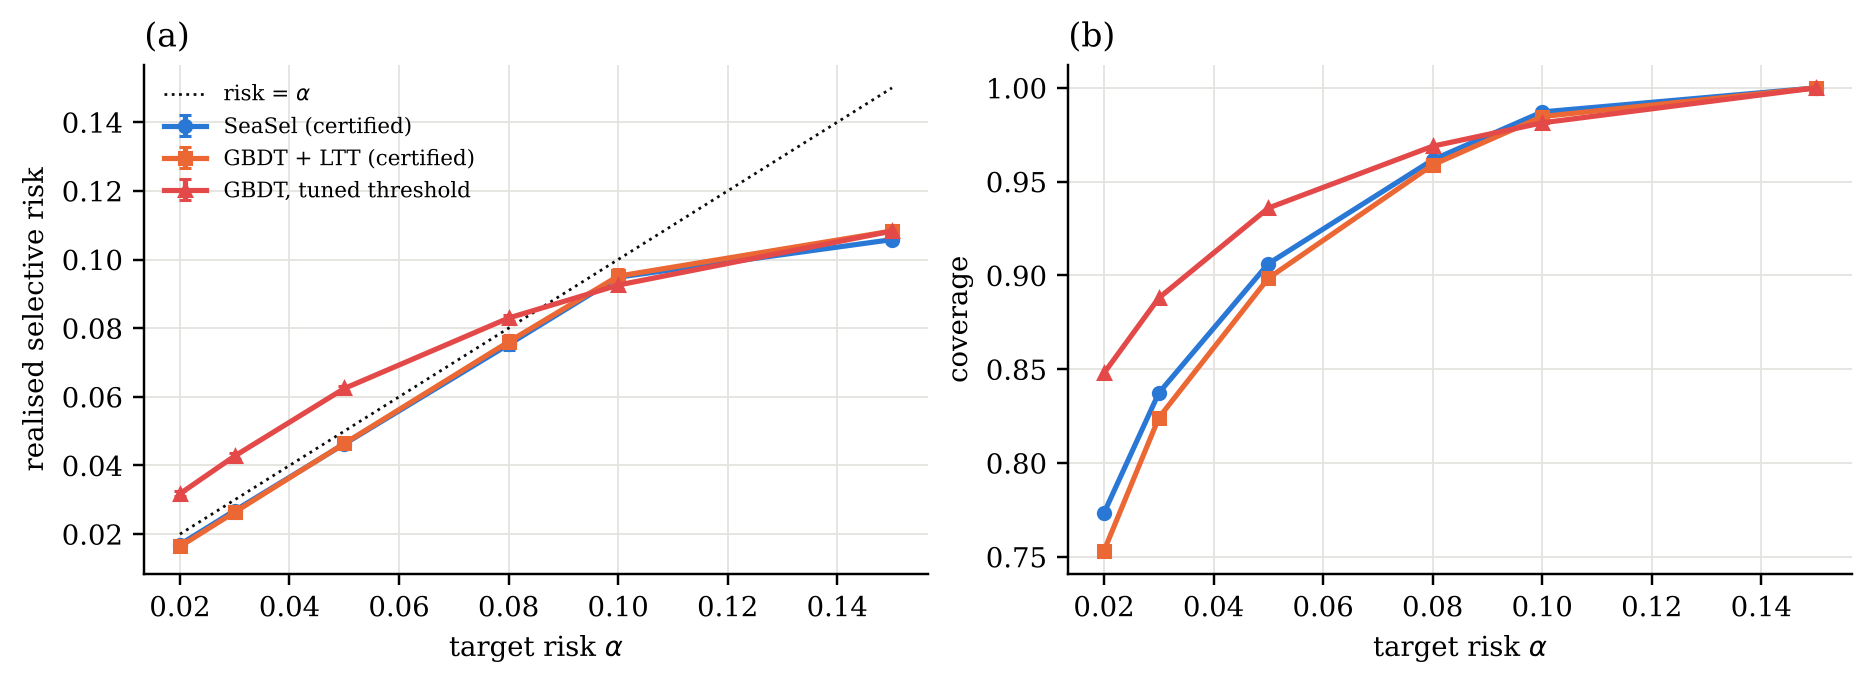
\includegraphics[width=0.95\textwidth]{../figures/fig_alpha_sweep.png}
\caption{\textbf{Guarantee validity across targets.} (\textbf{a}) Realised selective risk (mean $\pm$ s.d.\ over 60 splits) against the target $\alpha$; certified methods stay on or below the diagonal. (\textbf{b}) Coverage obtained at each target.}
\label{fig:alpha}
\end{figure}

% ===========================================================================
\section{Ablation, robustness, and OOD analyses}\label{sec:ablation}
% ===========================================================================
\subsection{Ablation}
Table~\ref{tab:ablation} removes one component at a time and retrains where necessary. The certificate keeps every variant within the target, so ablations affect only how many epochs can be accepted. Removing the link-history features (beacon deficit, blockage evidence) is by far the most damaging change: AUROC falls from \RSAuroc{} to \RAbNoHistAuroc{} and coverage from \RSCov\% to \RAbNoHistCov\%. The remaining components have small effects in distribution: removing the physics bias, replacing attention by mean pooling or by a per-link network, removing the motion context, removing the uncertainty penalty or temperature scaling, and using a single member each change coverage by less than one percentage point. In this testbed the previous beacon of each link already summarises most of the rain, blockage and motion state that the other features describe, so the per-link evidence dominates.

\begin{table}[t]\centering\small
\caption{\textbf{Ablation study} (retrained variants; $\alpha=0.05$, $\delta=0.1$, 100 splits).}
\label{tab:ablation}
\resizebox{\textwidth}{!}{\begin{tabular}{@{}lcccccc@{}}\toprule
Variant & AUROC & ECE & Coverage & Selective risk & Goodput (Mbit) & Viol.\\\midrule
\textbf{Full SeaSel} & 0.907 & 0.005 & 0.906 $\pm$ 0.002 & 0.046 $\pm$ 0.001 & 349.0 $\pm$ 0.5 & 0.01\\
Without physics bias (plain attention) & 0.906 & 0.006 & 0.905 $\pm$ 0.002 & 0.046 $\pm$ 0.001 & 348.5 $\pm$ 0.5 & 0.01\\
Mean pooling instead of attention & 0.907 & 0.007 & 0.908 $\pm$ 0.002 & 0.046 $\pm$ 0.001 & 349.6 $\pm$ 0.5 & 0.01\\
Without attention (per-link MLP) & 0.906 & 0.005 & 0.903 $\pm$ 0.002 & 0.046 $\pm$ 0.001 & 347.8 $\pm$ 0.5 & 0.01\\
Without motion and weather context & 0.906 & 0.009 & 0.906 $\pm$ 0.002 & 0.046 $\pm$ 0.002 & 349.1 $\pm$ 0.5 & 0.01\\
Without link-history features & 0.850 & 0.035 & 0.805 $\pm$ 0.005 & 0.046 $\pm$ 0.002 & 312.3 $\pm$ 1.3 & 0.02\\
Without uncertainty penalty (gamma = 0) & 0.907 & 0.005 & 0.907 $\pm$ 0.002 & 0.046 $\pm$ 0.002 & 349.2 $\pm$ 0.5 & 0.01\\
Without temperature scaling & 0.907 & 0.007 & 0.906 $\pm$ 0.002 & 0.046 $\pm$ 0.001 & 349.1 $\pm$ 0.5 & 0.01\\
Single member (M = 1) & 0.901 & 0.010 & 0.900 $\pm$ 0.002 & 0.046 $\pm$ 0.001 & 346.5 $\pm$ 0.5 & 0.02\\
\bottomrule\end{tabular}}\end{table}

\subsection{Cross-link transfer without history}
The value of reasoning across links appears when per-link evidence is missing, as for a satellite that has just risen or a terminal that has just restarted. Table~\ref{tab:transfer} retrains the three architectures with half of the satellite tokens lacking history and evaluates them in the same condition. On the tokens without history, physics-biased attention reaches an AUROC of \RTrPBAMiss, against \RTrATTMiss{} for plain attention and \RTrMLPMiss{} for the per-link network, and it certifies the largest coverage (\RTrPBACov\% against \RTrATTCov\% and \RTrMLPCov\%). The ordering is consistent but the margins are small. The geometric prior helps the model borrow evidence from nearby links, but it is a refinement of the prediction rather than the source of the guarantee.

\begin{table}[t]\centering\small
\caption{\textbf{Cross-link transfer when half of the link histories are missing} (models retrained and evaluated with 50\% of satellite tokens lacking beacon history; $\alpha=0.05$).}
\label{tab:transfer}
\resizebox{\textwidth}{!}{\begin{tabular}{@{}lcccccc@{}}\toprule
Predictor & AUROC (all) & AUROC (no history) & ECE & AURC & Coverage & Selective risk\\\midrule
Physics-biased attention & 0.881 & 0.858 & 0.015 & 0.0160 & 0.874 $\pm$ 0.003 & 0.046 $\pm$ 0.002\\
Plain attention & 0.879 & 0.854 & 0.016 & 0.0161 & 0.872 $\pm$ 0.003 & 0.046 $\pm$ 0.002\\
Per-link MLP & 0.878 & 0.850 & 0.018 & 0.0166 & 0.866 $\pm$ 0.004 & 0.046 $\pm$ 0.002\\
\bottomrule\end{tabular}}\end{table}

\subsection{Robustness to sensor corruption}
Table~\ref{tab:robust} corrupts the gateway inputs at test time. With the certificate obtained on clean data, inertial noise of 1--3$^\circ$, a threefold noisier rain gauge and 30\% missing context leave the selective risk below 5\%. Losing half of the link histories, however, raises it to 6.3\%, above the target, because the clean certificate no longer matches the input distribution. Recalibrating on data with the same corruption restores the target in every case; for missing histories this costs about four percentage points of coverage. Corruption of the history channel should therefore trigger recalibration or the online rule.

\begin{table}[t]\centering\small
\caption{\textbf{Robustness to sensor corruption at test time.} Fixed certificate from clean calibration versus recalibration on corrupted data ($\alpha=0.05$).}
\label{tab:robust}
\resizebox{\textwidth}{!}{\begin{tabular}{@{}lccccc@{}}\toprule
 & & \multicolumn{2}{c}{Clean certificate} & \multicolumn{2}{c}{Recalibrated}\\
Corruption & AUROC & Coverage & Selective risk & Coverage & Selective risk\\\midrule
IMU noise 1 deg & 0.897 & 0.918 & 0.040 & 0.931 & 0.045\\
IMU noise 3 deg & 0.875 & 0.847 & 0.027 & 0.915 & 0.045\\
Rain sensor noise x3 & 0.900 & 0.923 & 0.043 & 0.930 & 0.045\\
30\% context missing & 0.898 & 0.936 & 0.048 & 0.928 & 0.045\\
50\% link history missing & 0.874 & 0.947 & 0.063 & 0.903 & 0.045\\
\bottomrule\end{tabular}}\end{table}

\subsection{Out-of-distribution operation}
Table~\ref{tab:ood} and Fig.~\ref{fig:ood} evaluate three shifted days with the certificate obtained in distribution. Distribution shift breaks the in-distribution guarantee in all three cases: the selective risk rises to \RStormNaive\% on the severe-storm day, \RTropNaive\% on the tropical day and \RConstNaive\% when 30\% of satellites have failed. The sea-state-conditional certificate restores the target under storms (\RStormMond\%), where the shift is captured by the roll-RMS groups, but not under tropical rain or constellation loss, whose shifts are unrelated to sea state. The online rule (\ref{eq:online}) restores the target in all three cases (\RStormOnline\%, \RTropOnline\% and \RConstOnline\%) by lowering coverage to \RStormOnlineCov\%, \RTropOnlineCov\% and \RConstOnlineCov\%. Its coverage is close to that of an oracle that recalibrates on the shifted day itself. Figure~\ref{fig:ood}b shows the mechanism on the storm day: the fixed certificate lets the running risk climb to about 12\% at the height of the storm, whereas the online threshold keeps it near 5\% throughout. Always-aggressive operation would have lost \RStormAAMiss\% of critical messages on this day.

\begin{table}[t]\centering\small
\caption{\textbf{Out-of-distribution operation} (target $\alpha=0.05$). Sel.: selective risk; Cov.: coverage; Miss: critical-message miss rate.}
\label{tab:ood}
\resizebox{\textwidth}{!}{\begin{tabular}{@{}lcccccccccc@{}}\toprule
 & & \multicolumn{2}{c}{Always aggressive} & \multicolumn{2}{c}{In-distribution certificate} & \multicolumn{2}{c}{Sea-state conditional} & \multicolumn{2}{c}{Online adaptive}\\
Shift & AUROC & Sel. & Miss & Sel. & Cov. & Sel. & Cov. & Sel. & Cov.\\\midrule
Severe storms & 0.948 & 0.312 & 31.2\% & 0.057 & 0.687 & 0.048 & 0.661 & 0.049 & 0.670\\
Tropical rain & 0.906 & 0.128 & 12.8\% & 0.058 & 0.913 & 0.057 & 0.909 & 0.049 & 0.890\\
30\% satellite loss & 0.906 & 0.190 & 19.0\% & 0.101 & 0.877 & 0.101 & 0.867 & 0.050 & 0.757\\
\bottomrule\end{tabular}}\end{table}

\begin{figure}[t]
\centering
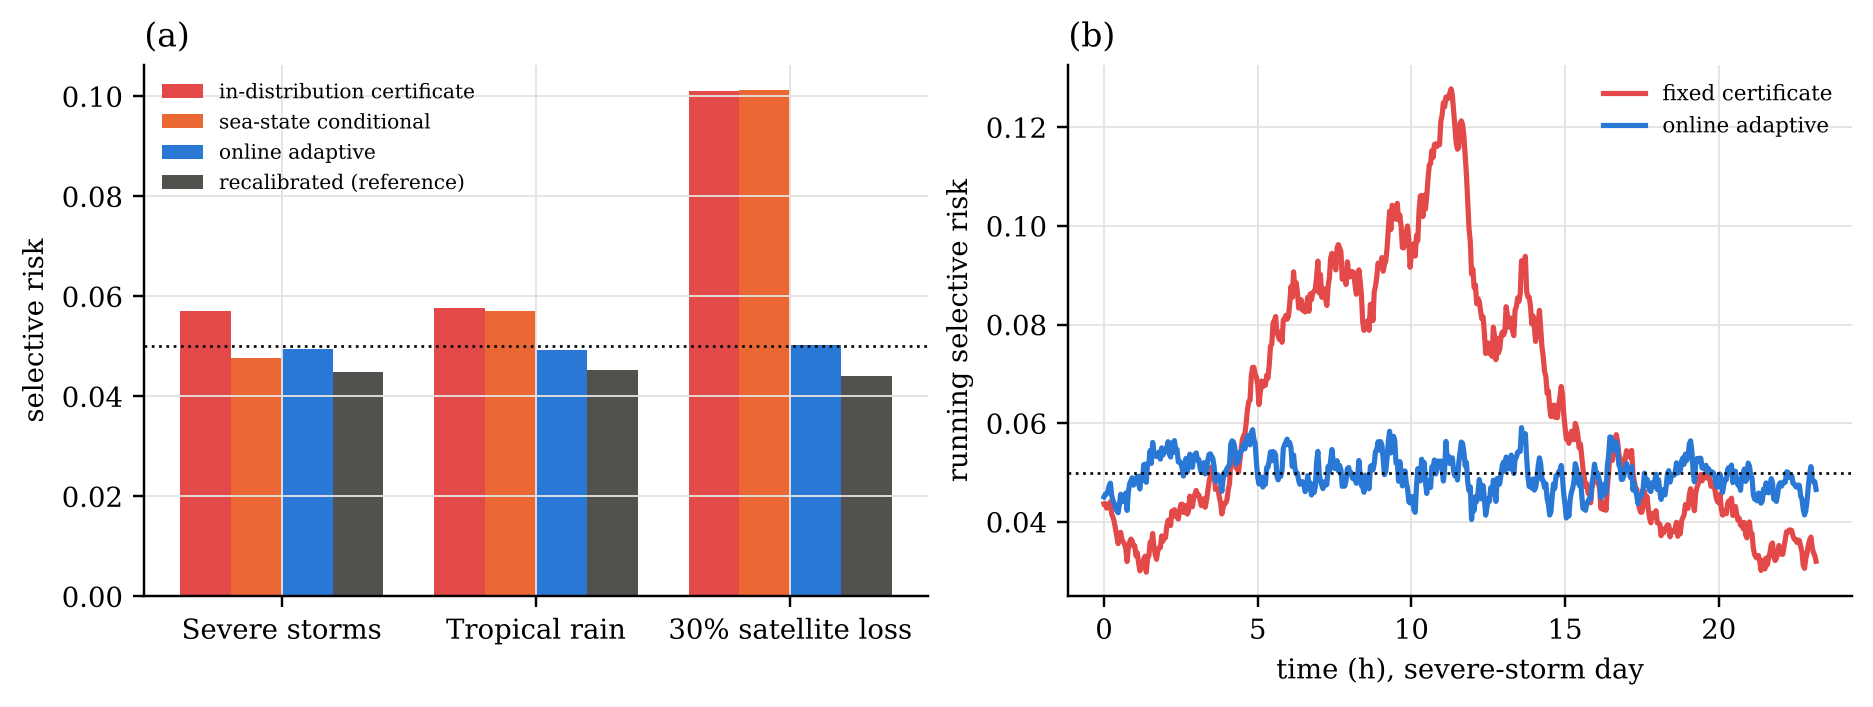
\includegraphics[width=0.95\textwidth]{../figures/fig_ood.png}
\caption{\textbf{Operation under distribution shift.} (\textbf{a}) Selective risk on three shifted days for the in-distribution certificate, the sea-state-conditional certificate, the online rule and an oracle recalibrated on the shifted day. (\textbf{b}) Running selective risk over the severe-storm day for the fixed certificate and the online rule. The dotted line marks $\alpha=0.05$.}
\label{fig:ood}
\end{figure}

% ===========================================================================
\section{Discussion, operational utility, and limitations}\label{sec:discussion}
% ===========================================================================
The results show that the main value of SeaSel lies in its decision interface rather than in its predictor. A certified threshold turns any well-calibrated link predictor into a policy with a verifiable reliability level. For a fleet operator this means alarm and safety telemetry can be given a contractual miss rate while bulk data still travel at near-aggressive rates, with no extra satellite capacity. The certificate is cheap: one calibration run per window, and \RMsDec{}\,ms per decision. The same mechanism applies to other risk-sensitive decisions on a vessel gateway, such as choosing a modulation order, scheduling handovers or deciding when to store and forward. Three limitations remain. First, all results come from a simulated testbed; field logs from vessels are needed to confirm the channel and motion models, although the certificate itself remains valid for any data that satisfy its exchangeability assumption. Second, the guarantee holds only under exchangeability, so drift must be handled by recalibration or by the online rule, whose guarantee is asymptotic. Third, the architectural gains of physics-biased attention are modest in distribution; larger fleets, richer beam-level telemetry and three-dimensional ray geometry may increase them.

% ===========================================================================
\section{Conclusion}\label{sec:conclusion}
% ===========================================================================
This paper introduced SeaSel, a framework that lets a vessel gateway act on learned satellite-link predictions only when a finite-sample certificate guarantees that accepted decisions rarely fail. The framework combines a physics-biased attention ensemble over all candidate links, a Learn-then-Test certificate with exact binomial p-values, a dual-link robust fallback with an explicit service-level bound, and sea-state-conditional and online variants for distribution shift. On a sandbox testbed with a two-shell constellation, storms, ship motion and blockage, SeaSel held the selective risk at \RSRisk\% for a 5\% target and cut critical-message misses by \RMissRed\% without losing goodput. Uncertified thresholds violated the target in almost every split. Under storms, tropical rain and constellation degradation, the online rule restored the target where the fixed certificate failed. The results also show where the gains come from: link history is the most informative input, calibration quality determines how many epochs can be certified, and drift is the main threat to the guarantee. Future work will validate the framework on field logs from vessels, extend it to multi-vessel coordination and inter-satellite routing, and study certificates that adapt to sea state, season and constellation health together.
